\documentclass[10pt]{article}
\usepackage[letterpaper, margin=1in]{geometry}
\usepackage[pdftex]{graphicx}
\usepackage[utf8]{inputenc}
\usepackage{tikz, wrapfig, amssymb, array, mathtools, circuitikz, physics, parskip, hyperref}
\usepackage{enumerate}
\usepackage{tkz-euclide}
\usepackage{titlesec}
\usepackage{lipsum}
\usepackage[english]{babel}
\usepackage{amsmath, amsthm}
\usepackage{fancyhdr}
\usepackage{xcoffins}
\usepackage{tcolorbox}
\usepackage{../local}


\newcommand{\classcode}{Physics 137A}
\newcommand{\classname}{Quantum Mechanics}
\renewcommand{\maketitle}{%
\hrule height4pt
\large{Eric Du \hfill \classcode}
\newline
\large{HW 09} \Large{\hfill \classname \hfill} \large{\today}
\hrule height4pt \vskip .7em
\normalsize
}
\linespread{1.1}
\begin{document}
    \maketitle

    \section*{Collaborators} 

    I worked with \textbf{Andrew Binder} to complete this assignment. 
    \section*{Problem 1}

    A particle with magnetic moment $\hat \mu$ is placed in a magnetic field $\mathbf{B}$. As a result, it has energy 

    \[ \hat H = -\hat \mu \cdot \mathbf B\]

    The magnetic moment of an electron (which is spin $\frac{1}{2}$) is related to its spin by its gyromagnetic ratio $\gamma$ (which has units of charge over mass):

    \[ \hat \mu = \gamma \hat{\mathbf S}\] 

    We will perform this problem in the $S_x$ eigenbasis: $\ket{+z}$ has eigenvalue $+\hbar/2$ and $\ket{-z}$ has eigenvalue $-\hbar/2$. 

    \begin{enumerate}[(a)]
        \item If we orient the magnetic field such that $\mathbf B = B_0 \hat{\mathbf z}$, (here $\hat{\mathbf z}$ is a unit vector not an operator) what are the energy eigenstates and eigenvalues?
        
        \begin{solution}
            The eigenvalues and eigenstates are $\ket{\pm z}$ with eigenvalues $\pm \hbar/2$, because the magnetic field is oriented in the $\hat z$ direction.
        \end{solution}
        \item If we orient the magnetic field in another direction, but we do not change its magnitude, argue why the energy eigenvalues are the same. 
        
        \begin{solution}
            The energy eigenvalues should not depend on the direction we poin the magnetic field in, but solely based on the magnitude, because that determines the strength of the magnetic field. 
        \end{solution}
        \item Let us orient the magnetic field such that $\mathbf B = B_0 \hat{\mathbf n}$, where 
        \[ \hat{\mathbf n} = \sin \theta \cos \phi \hat{\mathbf x} + \sin \theta \sin \phi \hat{\mathbf y} + \cos \theta \hat{\mathbf z}\] 

        Again, $\hat{\mathbf n}, \hat{\mathbf x}, \hat{\mathbf y}, \hat{\mathbf z}$ are unit vectors and not operators. Show that the energy eigenstates are given as

        \begin{align*}
            \ket{+n} &= \cos(\theta/2) \ket{+z} + e^{i\phi} \sin(\theta/2) \ket{-z}\\
            \ket{-n} &= \sin(\theta/2) \ket{+z} - e^{i\phi}\cos(\theta/2)\ket{-z}
        \end{align*}

        \begin{solution}
            The hint in part (e) states that the state: 

            \[ \cos \frac \theta 2 \ket{+z} + e^{i \phi} \ket{-z}\] 

            is at $(\theta, \phi)$, so using that, since we know that $\ket n$ can also be characterized as a unit vector with spherical coordinates $(1, \theta, \phi)$, then we can certainly express $\ket{+n}$ as: 

            \[ \ket{+n} = \cos(\theta/2) \ket{+z} + e^{i\phi} \sin(\theta/2) \ket{-z}\] 

            Then, $\ket{-n}$ is simply the opposite of this, where the $\ket{+z}$ term is now $\cos(\pi - \frac{\theta}{2}) = \sin \frac{\theta}{2}$ and likewise $\sin \pi - \frac \theta 2 = \cos \frac \theta 2$, and therefore: 

            \[ \ket{-n} = \sin(\theta/2) \ket{+z} - e^{i\phi}\cos(\theta/2)\ket{-z}\] 
        \end{solution}
        \item The state $\ket{+n}$ gives us a way to map from the surface of a sphere, parametrised by $(\theta, \phi)$, to the space of physical state of a two-level quantum mechanical system, 
        \[ \ket{\psi(\theta, \phi)} = \cos(\theta/2)\ket{+z} + e^{i\phi}\sin(\theta/2)\ket{-z}\] 

        Show that this is a bijection between the sphere and space of physical states. that is, show that any normalized state of a two-level system can be uniquely determined by a point on a sphere with coordinates $(\theta, \phi)$. [Hint: Begin by showing that any two-level state is equivalent to a $\ket{+n}$. Then show that all coordinate pairs $(\theta, \phi)$ that refer to the same point on a sphere also refer to the same quantum state]. We call the sphere made of these points the Bloch sphere

        \begin{solution}
            Becasue $\theta, \phi$ is a orthogonal and complete set of coordinates on a sphere of radius 1, then any vector $\ket{+n}$ can be expressed in terms of $(\theta, \phi)$.
        \end{solution}
        \item Draw the Bloch sphere and place points indicating where the eigenstates of $S_x$, $S_y$ and $S_z$ are mapped to. [Hint: the state
        \[ \cos \frac{\theta}{2} \ket{+z} + e^{i\phi} \sin \frac \theta 2 \ket{-z}\]
        is at the coordinate $(\theta, \phi)$]

        \begin{solution}
            The Bloch sphere is sipmly a unit sphere pointing in the direction $(\theta, \phi)$, with the $+z$ axis with state $\ket{+z}$ (or $\ket 0$) and with the $-z$ axis with the state $\ket{-z}$ (or $\ket 1$):


            \begin{center}
                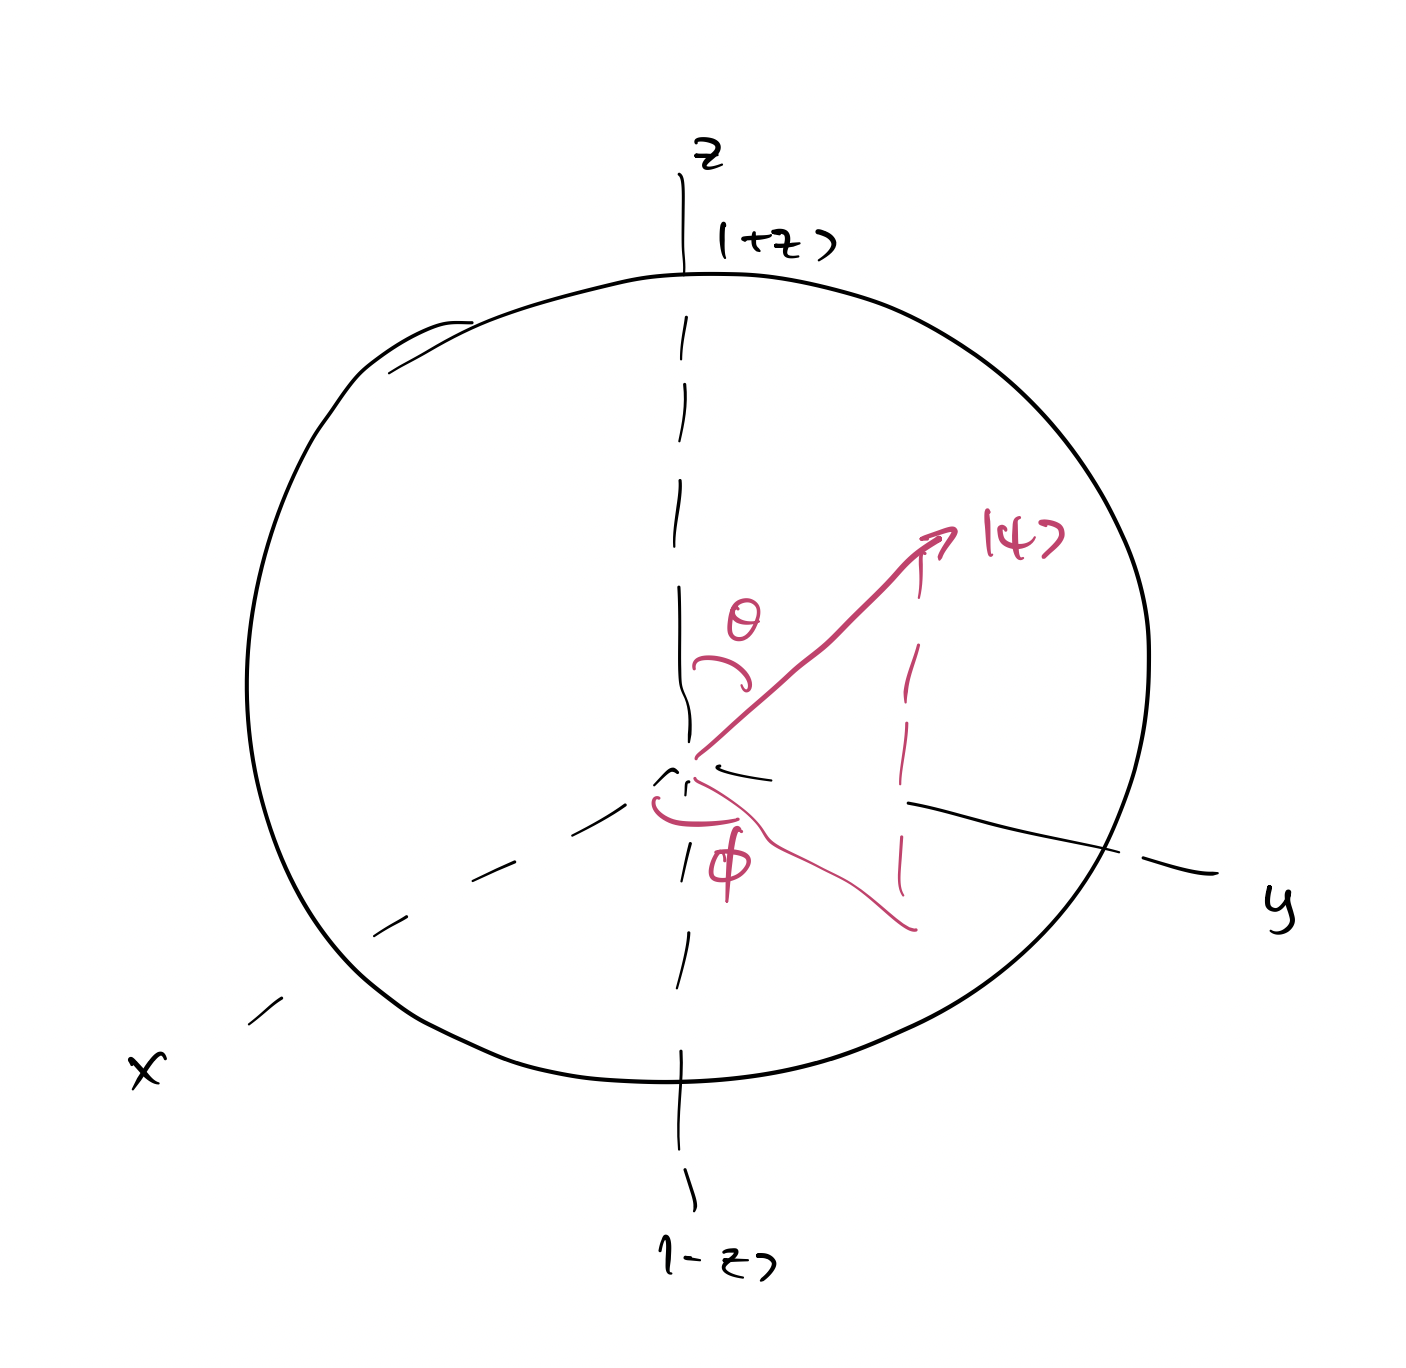
\includegraphics[scale=0.5]{bloch.png}
            \end{center}
        \end{solution}
        \item Calculate $\mean{S_x}$, $\mean{S_y}$ and $\mean{S_z}$ for the state $\ket{\psi(\theta, \phi)}$. 
        
        \begin{solution}
            I suppose here, we would simply plug these into our normal equations for the expected value:

            \[ \mean{\hat A} = \expval{\hat A}{\chi}\]

            And so therefore this would mean 

            \[ \mean{S_i} = \expval{S_i}{\chi}, \phantom{aa} i = x, y, z\]

            This is likely most easily done using the matrix representations of $S_x$, $S_y$ and $S_z$.
        \end{solution}
        

    \end{enumerate}

    \pagebreak

    \section*{Problem 2}

    Do this problem after problem 1. It will make more sense that way. 

    \begin{enumerate}[(a)]
        \item If we rotate the $\ket{+z}$ state around the $\hat{\mathbf x}$ axis by angle $\varphi$, what will it become? What about $\ket{-z}$? [Hint: Make use of the physical connection from the previous problem. If a state was in the $\ket{+z}$ state, it would have a specific energy when a magnetic field is pointing in the $\hat{\mathbf z}$ direction. If we rotate out (unphysical) coordinates so that the magnetic field points in the $\hat n$ direction, the state must still have the same energy, and the state that has that energy is $\ket{+n}$. So, if we rotate $\hat{\mathbf z}$ to $\hat{\mathbf n}$, then $\ket{+z}$ becomes $\ket{+n}$]
        
        \begin{solution}
            If we rotate the $\ket{+z}$ state around by an angle $\varphi$, it also makes sense to rotate the $\ket{-z}$ state around by an angle $-\varphi$, so that the state preserves the same amount of energy. Therefore, since from the previous problem we confirmed that a state $\ket{n}$ can be written as: 
            \[ \ket{+n} = \cos(\theta/2) \ket{+z} + e^{i\phi} \sin(\theta/2) \ket{-z}\]

            Then all we need to do is add in this change in $\phi \to \phi - \varphi$: 

            \[ \ket{+n} = \cos(\theta/2) \ket{+z} + e^{i(\phi + \varphi)} \sin(\theta/2) \ket{-z}\]

            And likewise, 

            \[ \ket{-n} = \sin(\theta/2) \ket{+z} - e^{i(\phi - \varphi)}\cos(\theta/2)\ket{-z}\] 

        \end{solution}
        \item Use the above result to find the matrix representation (in the $S_x$ eigenbasis) of the operator $\hat R(\phi \hat{\mathbf x})$ that rotates a spin state around the $\hat{\mathbf x}$-axis by an angle $\varphi$.
        
        \begin{solution}
            We would assemble the matrix of $\hat R$ by finding all the rotation factors (and also normalized) then plug them into a matrix.
        \end{solution}
    \end{enumerate}

    \pagebreak

    \section*{Problem 3}

    Use separation of variables in \textit{cartesian} coordinates to solve the infinite cubical well (or ``particle in a box''):

    \[ V(x, y, z) = \begin{cases}
        0, & \text{if $x, y, z$ are all between 0 and $a$}\\
        \infty, & \text{otherwise}
    \end{cases}\]

    \begin{enumerate}[(a)]
        \item Find the stationary states, and the corresponding energies
        
        \begin{solution}
            The stationary states are separable solutions, so from lecture, we know that the 3D wavefunction that satisfies these properties is:

            \[ \psi_{n_x, n_y, n_z}(x, y, z) = \sqrt{\frac{8}{L_1L_2L_3}} \sin \left(\frac{n_x \pi x}{L_1}\right) \sin\left(\frac{n_y \pi y}{L_2}\right) \sin \left(\frac{n_z\pi y}{L_3}\right)\] 

            Here in this problem, we have $L_1 = L_2 = L_3 = a$, so our solution simplifies to: 

            \[ \psi_{n_x, n_y, n_z}(x,y,z) = \sqrt{\frac{8}{a^3}} \sin\left(\frac{n_x \pi x}{a}\right) \sin\left(\frac{n_y \pi x}{a}\right) \sin\left(\frac{n_z \pi z}{a}\right)\]

            Their associated energies are: 

            \[ E = \frac{\hbar^2 \pi^2}{2ma^2}(n_x^2 +n_y^2 + n_z^2)\]
        \end{solution}
        \item Call the distinct energies $E_1, E_2, E_3, \dots$, in order of increasing energy. Find $E_1, E_2, E_3, E_4, E_5$ and $E_6$. Determine their degeneracies (that is, the number of different states that share the same energy). \textit{Comment:} In \textit{one} dimension degenerate bound states do not occur (see Problem 2.45), but in three dimensions they are very common. 
        
        \begin{solution}
            From lecture, we know that $E_1$ has only one degeneracy: $(1, 1, 1)$. For $E_2$, we have three: $(2, 1, 1), (1, 2, 1), (1, 1, 2)$, and $E_3$ has 3: $(2, 2, 1), (2, 1, 2), (1, 2, 2)$. 

            We continue this way to generate the following table: 

            \begin{center}
                \begin{tabular}{l|l|l}
                    Energy $E/E_0$ & $(n_x, n_y, n_z)$                        & Degeneracy \\ \hline
                    1              & $(1, 1, 1)$                              & $d = 1$    \\ \hline
                    2              & $(2, 1, 1), (1, 2, 1), (1, 1, 2)$        & $d = 3$    \\ \hline
                    3              & $(2, 2, 1), (2, 1, 2), (1, 2, 2)$        & $d = 3$    \\ \hline
                    11/3           & $(3, 1, 1), (1, 3, 1), (1, 1, 3)$        & $d = 3$    \\ \hline
                    4              & $(2, 2, 2)$                              & $d = 1$    \\ \hline
                    14/3           & $(1, 2, 3), (1, 3, 2), (2, 3, 1), \dots$ & $d = 6$   
                    \end{tabular}
            \end{center}
        \end{solution}
        \item What is the degeneracy of $E_{14}$, and why is this case interesting?
        
        \begin{solution}
            $E_{14}$ would be the fourteenth smallest combinatorial sum of three squares, which ends up requiring the sum of $n_x^2 + n_y^2 + n_z^2 = 27$ (the 14th number of sequence A000408 in the OEIS). This case is paritcularly interesting because there are two sets of numbers $(3, 3, 3)$ and $(5, 1, 1)$ which both sum fo 27, so we have to take the sum of both of these degeneracies, which we get to be 4.
        \end{solution}
    \end{enumerate}


    \pagebreak

    \section*{Problem 4}

    Consider the \textbf{three-dimensional harmonic oscillator}, for which the potential is

    \[ V(r) = \frac{1}{2} m\omega^2r^2\] 

    \begin{enumerate}[(a)]
        \item Show that separation of variables in cartesian coordinates turns this into three one-dimensional oscillators, and exploit your knowledge of the latter to determine the allowed energies. \textit{Answer:}
        \[ E_n = (n+ 3/2)\hbar \omega\]

        \begin{solution}
            The quantum harmonic oscillator is also separable into three one-dimensional oscillators in the $x, y$ and $z$ directions, so therefore: 

            \[ E_i = \left(n + \frac 12\right) \hbar \omega, \phantom{aa} i = x, y, z\]

            And so therefore we take the sum total of these: 

            \[ E = (n_x+ n_y + n_z + \frac 32) \hbar \omega\]

            We could then define $n = n_x + n_y + n_z$ to get the desired answer in the problem statement.
        \end{solution}
        \item Determine the degeneracy $d(n)$ of $E_n$.
        
        \begin{solution}
            The degeneracy of $E_n$ is tied to $n$, and to determine $n_x, n_y, n_z$ we simply run through all possible ways of summing $n$ using three numbers. Therefore, this becomes a purely combinatorial problem. Then, we need to reindex $n \to n+1$ because $n$ starts at 0, we get: 

            \[ d(n) = {n+2 \choose 2} = \frac{(n+2)(n+1)}{2}\]
        \end{solution}
    \end{enumerate}
\end{document}